\section{Validação de Cálculos e Especificação de Retornos}

Dentre as etapas fundamentais no desenvolvimento de \textit{softwares}, a fase de testagem apresenta papel de grande relevância, uma vez que possibilita a verificação sistemática da conformidade dos resultados obtidos com aqueles previstos teoricamente. No contexto deste trabalho, essa etapa é essencial para garantir a confiabilidade dos cálculos e das rotinas computacionais empregadas em aplicações de Engenharia Química.

Uma abordagem eficiente para a realização desses testes consiste na utilização da biblioteca \textit{pytest}, que permite a implementação de testes automatizados desenvolvidos para assegurar o correto funcionamento dos módulos do sistema. Por meio dessa ferramenta, é possível validar, de forma reprodutível e padronizada, os retornos das funções responsáveis pelos cálculos de propriedades, balanços e demais operações recorrentes da área.

Com o objetivo de detalhar o funcionamento do \textit{software} desenvolvido, as funcionalidades de cada módulo são descritas a seguir, acompanhadas de evidências da interface \textit{frontend} e de instruções para o consumo direto das rotinas por meio da linguagem \textit{Python}, permitindo tanto a utilização via interface gráfica quanto a integração do sistema com outros projetos e aplicações computacionais.

\subsection{Componentes}

Para iniciar a biblioteca local com o módulo de componentes, o código da figura abaixo deve ser inserido, assegurando que o \textit{Python} consiga identificar as funções dentro da classe \textit{Components} contida no arquivo \textit{./models/componentes.py}.

Tendo que o passo a passo para consumir via \textit{API} ou \textit{Python} o projeto seja demasiado técnico, será apenas brevemente comentado abaixo o modo de se fazer, depois havendo maior realce apenas aos retornos e comentários correlatos.

\begin{figure}[H]
    \centering
    \caption{Inicialização da biblioteca de componentes via \textit{Python}}
    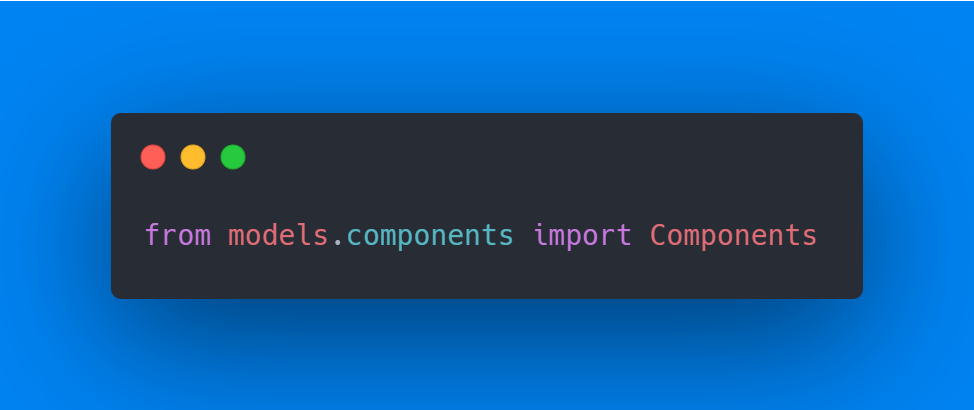
\includegraphics[width=\linewidth]{media/cap4_inicializacao_biblioteca_componentes_python.png}
    \fonte{Elaboração própria (2026).}
\end{figure}

No \textit{frontend}, basta acessar a aba \textit{Components} e rolar a página para visualizar as funcionalidades.

\begin{figure}[H]
    \centering
    \caption{Inicialização da biblioteca de componentes via \textit{frontend}}
    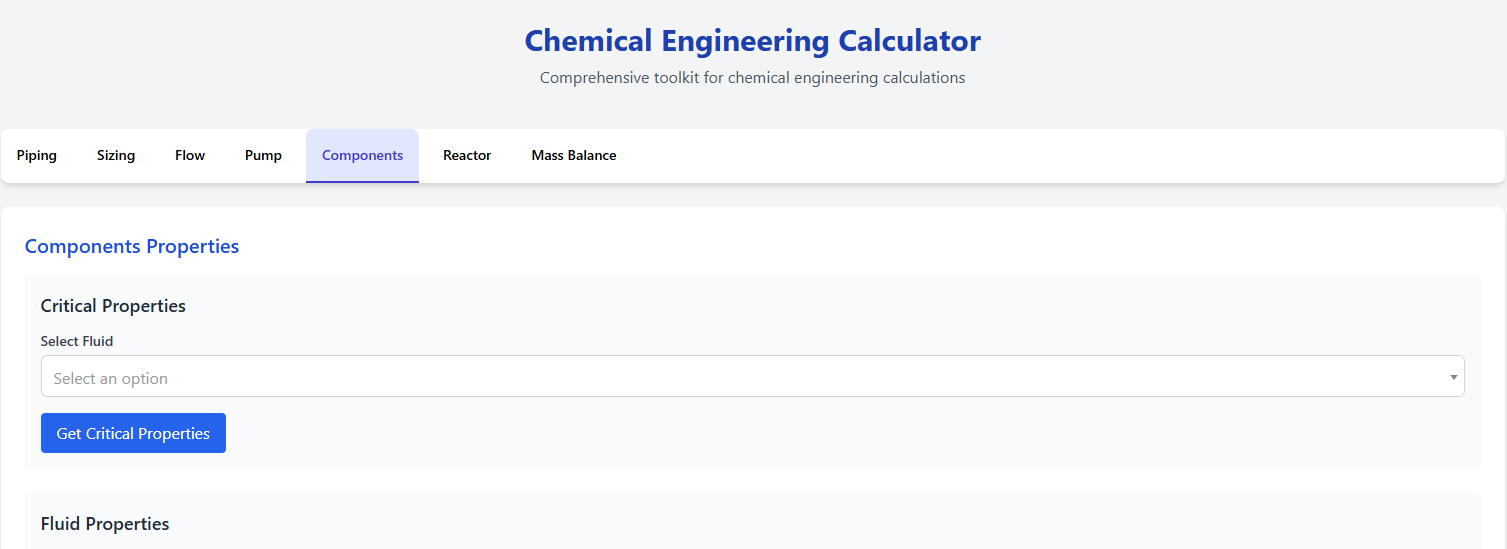
\includegraphics[width=\linewidth]{media/cap4_inicializacao_biblioteca_componentes_frontend.png}
    \fonte{Elaboração própria (2026).}
\end{figure}

\subsubsection{Listar Componentes}

A função \textit{list\_all\_components()} interage diretamente com a biblioteca termodinâmica \textit{CoolProp} para listar todas as substâncias puras e pseudo-puras disponíveis para cálculo. O teste retornou um total de 124 fluidos cadastrados, abrangendo desde hidrocarbonetos simples e refrigerantes até fluidos inorgânicos como água e amônia. Esta listagem valida a capacidade do sistema em operar com uma vasta gama de componentes químicos industriais.

\begin{figure}[H]
    \centering
    \caption{Listagem parcial de componentes disponíveis na biblioteca termodinâmica}
    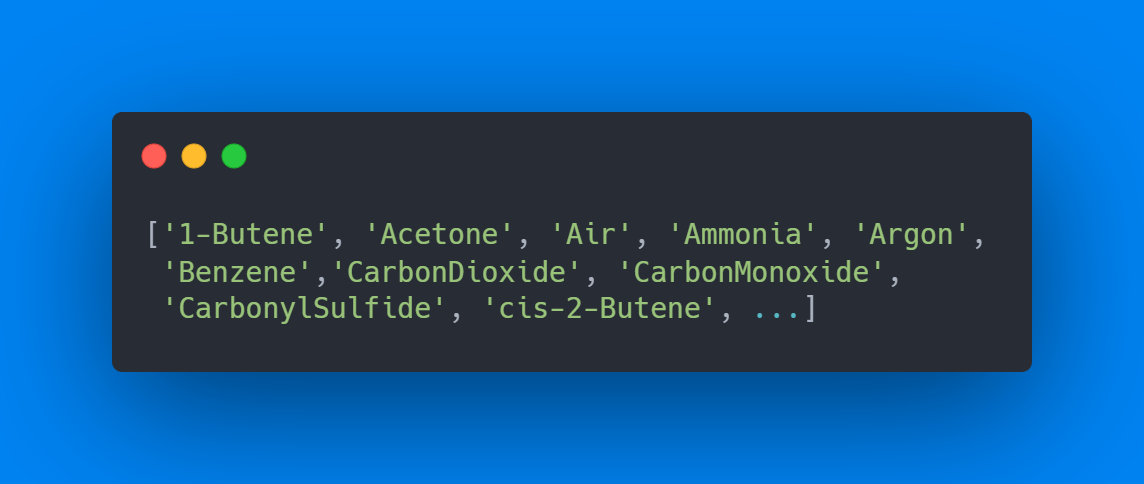
\includegraphics[width=\linewidth]{media/cap4_listagem_componentes_termodinamica.png}
    \fonte{Elaboração própria (2026).}
\end{figure}

\subsubsection{Valor de Propriedade}

Ao solicitar as propriedades termofísicas para o componente \textit{Water} (água) nas condições de $300\ \mathrm{K}$ e $101325\ \mathrm{Pa}$ ($1\ \mathrm{atm}$), o sistema retornou valores consistentes com a literatura. A massa específica calculada foi de $996{,}56\ \mathrm{kg/m^3}$ e a viscosidade de $8{,}54 \cdot 10^{-4}\ \mathrm{Pa \cdot s}$. Nota-se que o retorno inclui explicitamente as unidades físicas, utilizando a biblioteca \textit{Pint}, garantindo a consistência dimensional dos cálculos subsequentes.

\begin{figure}[H]
    \centering
    \caption{Propriedades termofísicas da água calculadas a 300K e 101,3kPa.}
    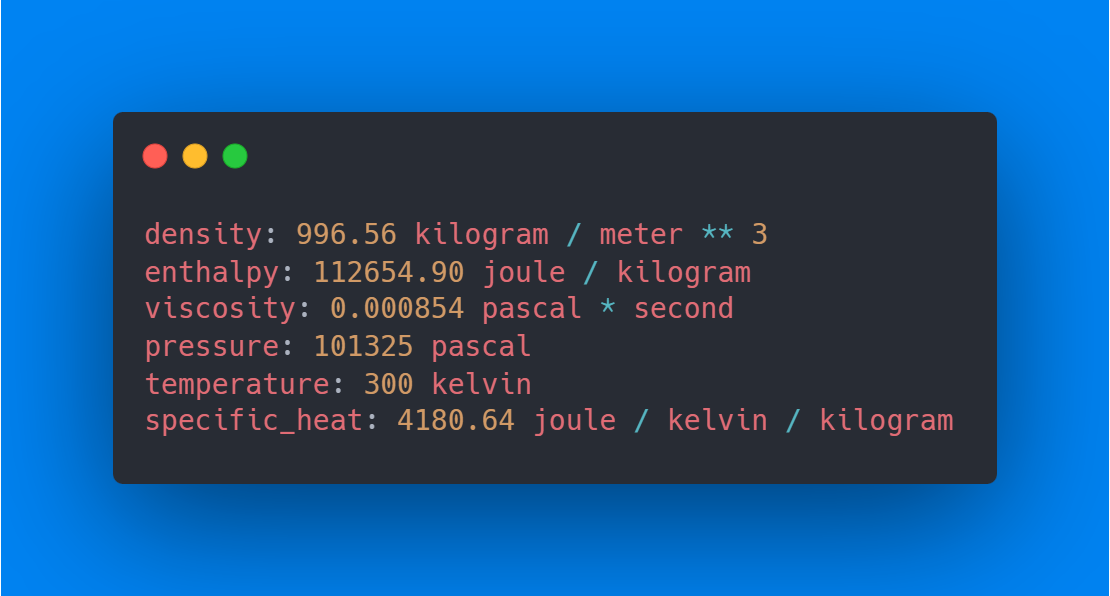
\includegraphics[width=\linewidth]{media/cap4_propriedades_agua_300k_101_3kpa.png}
    \fonte{Elaboração própria (2026).}
\end{figure}

\subsubsection{Nome de Propriedades}

A função \textit{get\_property\_names()} expõe o mapeamento interno entre as chaves de solicitação da \textit{API} (como 'D', 'H', 'V') e suas respectivas descrições físicas e unidades no SI. Esta estrutura organizacional permite que o usuário identifique rapidamente quais variáveis termodinâmicas podem ser requisitadas ao modelo, facilitando a configuração de simulações de balanço de massa e energia.

\begin{figure}[H]
    \centering
    \caption{Mapeamento de chaves de propriedades e suas unidades padronizadas.}
    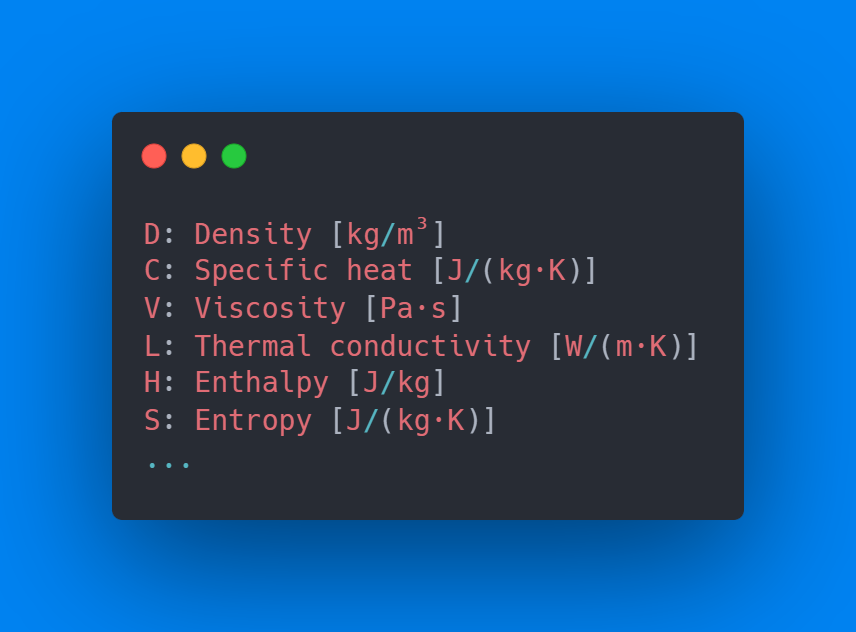
\includegraphics[width=\linewidth]{media/cap4_mapeamento_chaves_unidades.png}
    \fonte{Elaboração própria (2026).}
\end{figure}

\subsubsection{Propriedades Críticas}

A consulta das propriedades críticas para a água retornou uma temperatura crítica ($T_{c}$) de $647{,}1\ \mathrm{K}$ e uma pressão crítica ($P_{c}$) de $22{,}06\ \mathrm{MPa}$. Esses parâmetros fixos são fundamentais para o cálculo de propriedades reduzidas e para a verificação dos limites de fase da substância nas equações de estado. O sistema também forneceu os dados do ponto triplo, expandindo a utilidade da ferramenta para análises de equilíbrio de fases.

\begin{figure}[H]
    \centering
    \caption{Propriedades críticas e do ponto triplo calculadas para a água.}
    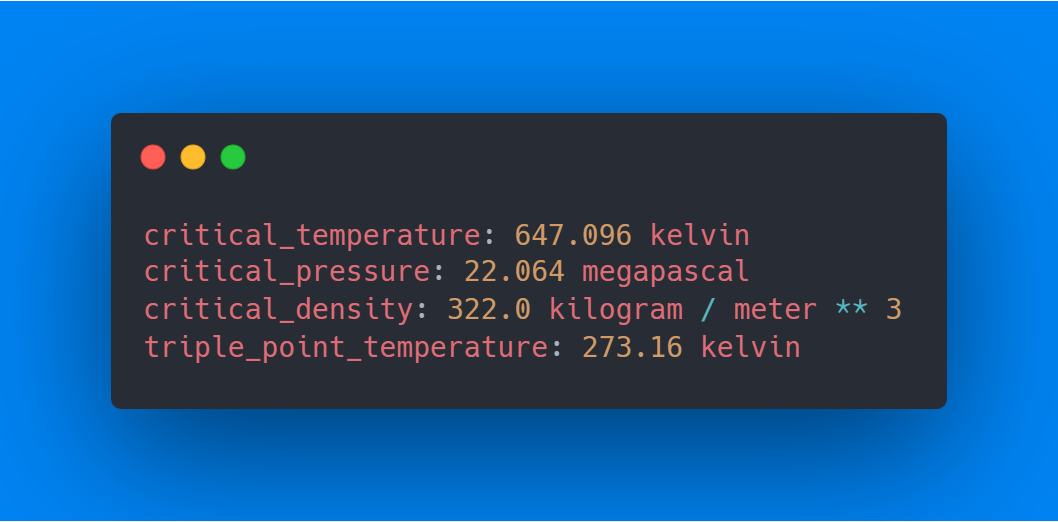
\includegraphics[width=\linewidth]{media/cap4_propriedades_criticas_ponto_triplo_agua.png}
    \fonte{Elaboração própria (2026).}
\end{figure}

\subsubsection{Opções de Propriedades de Misturas}

Para sistemas multicomponentes, a função \textit{get\_property\_mixture\_names()} delimita o subconjunto de propriedades que podem ser calculadas. Diferentemente das substâncias puras, observa-se que certas propriedades de transporte específicas ou tensão superficial podem não estar disponíveis dependendo do modelo de mistura (\textit{HEOS}) empregado. A listagem confirma a disponibilidade das variáveis de estado essenciais (entalpia, entropia, massa específica) necessárias para o dimensionamento de reatores e tubulações.

\begin{figure}[H]
    \centering
    \caption{Propriedades termodinâmicas disponíveis para cálculo em misturas.}
    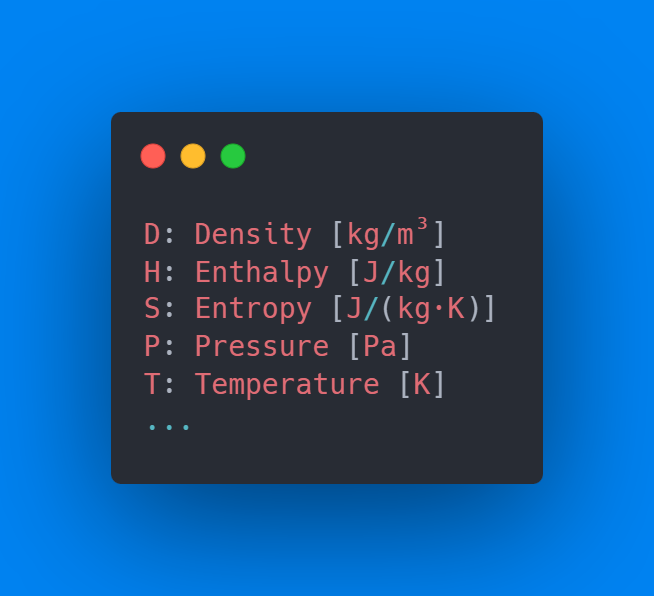
\includegraphics[width=\linewidth]{media/cap4_chaves_propriedades_mistura.png}
    \fonte{Elaboração própria (2026).}
\end{figure}

\subsubsection{Valor de Propriedades de Misturas}

A simulação de uma mistura binária equimolar de Água $( 5 0 \% )$ e Etanol ($5 0 \% )$a $3 0 0 K$ e $1 a t m$ resultou em uma massa específica de mistura de $8 1 4 , 0 4 \  k g / m^{3}$. O código utiliza internamente a regra de mistura baseada na energia livre de Helmholtz (HEOS) do \textit{CoolProp} para ponderar as interações moleculares entre os componentes. Este valor intermediário entre a massa específica da água pura ($9 9 7 k g / m^{3}$) e do etanol puro ($7 8 9 k g / m^{3}$) demonstra a eficácia do algoritmo em prever o comportamento não-ideal da solução.

\begin{figure}[H]
    \centering
    \caption{Propriedades termodinâmicas disponíveis para cálculo em misturas.}
    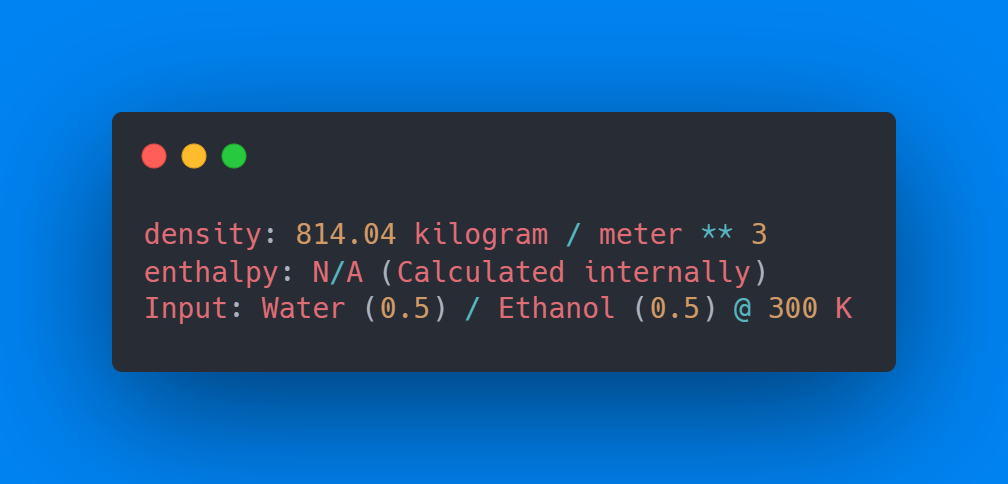
\includegraphics[width=\linewidth]{media/cap4_valores_propriedades_mistura.png}
    \fonte{Elaboração própria (2026).}
\end{figure}

\subsection{Hidráulicos}
\subsubsection{Perda de Carga}
Para a validação do cálculo de perda de carga, utilizou-se o método de Darcy--Weisbach, aplicável a fluxos incompressíveis em qualquer regime de escoamento. A equação base para o cálculo é a Equação \ref{eq:darcy}.

Nesta validação, comprimentos e diâmetros são tratados em metros, a velocidade em $m/s$, $g$ em $m/s^2$ e a perda de carga calculada $h_f$ é reportada em metros.

Onde a perda de carga localizada ($\sum h_{local}$) é calculada através do comprimento equivalente ($L_{eq}$) dos acessórios:

\begin{equation}
L_{total} = L + \sum (L_{eq} \cdot D)
\label{eq:val_len_total}
\end{equation}

\textbf{Teste A: Tubulação Reta (Sem Acessórios)}
\begin{itemize}
    \item \textbf{Dados:} $L=100m, D=50mm (0,05m), V=2,0m/s, f=0,02$
    \item \textbf{Cálculo Manual:}
    \begin{equation}
h_f = 0,02 \cdot \frac{100}{0,05} \cdot \frac{2^2}{2 \cdot 9,80665} = 40 \cdot 0,2039 = 8,1577 \ m
\label{eq:val_hf_calc_a}
\end{equation}
    \item \textbf{\textit{Software}:} $8,1577 \ m$
    \item \textbf{Status:} Resultado concordante, com desvio de 0,00\%.
\end{itemize}

\textbf{Teste B: Com Acessórios (2 Curvas 90º Raio Longo)}
\begin{itemize}
    \item \textbf{Dados Adicionais:} 2 Cotovelos ($L_{eq}/D = 16$).
    \item \textbf{Comprimento Equivalente:} $L_{eq} = 2 \cdot (16 \cdot 0,05) = 1,6 m$
    \item \textbf{Comprimento Total:} $101,6 m$
    \item \textbf{Cálculo Manual:}
    \begin{equation}
h_f = 0,02 \cdot \frac{101,6}{0,05} \cdot \frac{2^2}{2 \cdot 9,80665} = 8,2882 \ m
\label{eq:val_hf_calc_b}
\end{equation}
    \item \textbf{\textit{Software}:} $8,2882 \ m$
    \item \textbf{Status:} Resultado concordante, com desvio de 0,00\%.
\end{itemize}

\subsubsection{Reynolds}
O Número de Reynolds ($Re$) foi validado utilizando as duas formas de entrada suportadas pela \textit{API}: viscosidade dinâmica ($\mu$) e cinemática ($\nu$).

\textbf{Método 1: Viscosidade Dinâmica}
(Equação \ref{eq:reynolds_din})
\begin{itemize}
    \item \textbf{Dados:} $\rho=998 kg/m^3, V=2,0 m/s, D=0,05 m, \mu=1,002 \cdot 10^{-3} Pa \cdot s$
    \item \textbf{Cálculo Manual:} $Re = \frac{998 \cdot 2 \cdot 0,05}{0,001002} = 99.600,8$
    \item \textbf{\textit{Software}:} $99.600,8$
    \item \textbf{Status:} Resultado concordante, com desvio de 0,00\%.
\end{itemize}

\textbf{Método 2: Viscosidade Cinemática}
(Equação \ref{eq:reynolds_cin})
\begin{itemize}
    \item \textbf{Dados:} $V=2,0 m/s, D=0,05 m, \nu=1,004 \cdot 10^{-6} m^2/s$
    \item \textbf{Cálculo Manual:} $Re = \frac{2 \cdot 0,05}{1,004 \cdot 10^{-6}} = 99.601,6$
    \item \textbf{\textit{Software}:} $99.601,6$
    \item \textbf{Status:} Resultado concordante, com desvio de 0,00\%.
\end{itemize}

\subsubsection{Fator de Atrito}
O fator de atrito de Darcy ($f$) foi validado comparando métodos iterativos e explícitos.

\textbf{A. Consistência de Colebrook-White \cite{colebrook1939}}
Equação implícita (padrão, definida na Equação \ref{eq:colebrook}):
Verificou-se a convergência da solução numérica da \textit{API} comparando o Lado Esquerdo (\textit{LHS}) e Direito (\textit{RHS}) da equação.
\begin{itemize}
    \item \textbf{Dados:} $\varepsilon=0,045mm, D=50mm, Re=100.000$
    \item \textbf{\textit{Software} ($f$):} $0,021614$
    \item \textbf{Check:} \textit{LHS} = 6,802; \textit{RHS} = 6,802
    \item \textbf{Status:} Convergência confirmada.
\end{itemize}

\textbf{B. Equação de Swamee-Jain (Explícita) \cite{swamee1976}}
(ver Equação \ref{eq:swamee})
\begin{itemize}
    \item \textbf{Cálculo Manual:} $f = 0,02199$
    \item \textbf{\textit{Software}:} $0,02199$
    \item \textbf{Status:} Resultado concordante.
\end{itemize}

\textbf{C. Equação de Haaland (Explícita) \cite{haaland1983}}
(ver Equação \ref{eq:haaland})
\begin{itemize}
    \item \textbf{Cálculo Manual:} $f = 0,02161$
    \item \textbf{\textit{Software}:} $0,02161$
    \item \textbf{Status:} Resultado concordante.
\end{itemize}

\subsubsection{Diâmetro Real}
A função de seleção de diâmetro comercial verifica o próximo diâmetro nominal disponível numa tabela de \textit{Schedule}.

\begin{itemize}
    \item \textbf{Entrada:} Diâmetro Calculado = 45,0 mm. \textit{Schedule} = SCH40.
    \item \textbf{Lógica Manual:} Consultar tabela SCH40. Diâmetros disponíveis: ..., 32, 40, 50, 65... O próximo maior que 45 é 50.
    \item \textbf{\textit{Software}:} $50,0 \ mm$
    \item \textbf{Status:} Resultado concordante.
\end{itemize}

\subsubsection{Diâmetro Calculado}
O dimensionamento preliminar baseia-se na equação da continuidade para dutos circulares.

(ver Equação \ref{eq:diametro_calc})

\begin{itemize}
    \item \textbf{Dados:} $Q=0,005 m^3/s, V=1,5 m/s$
    \item \textbf{Cálculo Manual:} $D = \sqrt{\frac{4 \cdot 0,005}{\pi \cdot 1,5}} = \sqrt{0,004244} = 0,06515 \ m \ (65,15 mm)$
    \item \textbf{\textit{Software}:} $65,15 \ mm$
    \item \textbf{Status:} Resultado concordante, com desvio de 0,00\%.
\end{itemize}

\subsubsection{\textit{NPSH} Disponível}
O cálculo do \textit{Net Positive Suction Head} disponível ($NPSH_a$) utiliza a equação de Bernoulli aplicada à sucção da bomba:

\begin{center} Utilizando a Equação \ref{eq:npsh} \end{center}

\begin{itemize}
    \item \textbf{Dados:} $P_{man}=0{,}5\,\mathrm{kgf/cm^2}$, $P_{atm}=1\,\mathrm{atm}$, $P_{vap}=0{,}02\,\mathrm{kgf/cm^2}$, $\gamma=9806\,\mathrm{N/m^3}$, $h_f=1\,\mathrm{m}$, $\Delta Z=2\,\mathrm{m}$
    \item \textbf{Termos de Pressão (m.c.a):} $H_{press} = \frac{(0{,}5+1{,}033) \cdot 98.066{,}5}{9.806{,}6} = 15{,}33\,\mathrm{m}$, $H_{vap} = 0{,}2\,\mathrm{m}$
    \item \textbf{Cálculo Manual:} $15,33 + 2,0 + 0,11 - 1,0 - 0,2 = 16,24 \ m$
    \item \textbf{\textit{Software}:} $16,24 \ m$
    \item \textbf{Status:} Resultado concordante, com desvio inferior a 0,01\%.
\end{itemize}

\subsubsection{Altura manométrica}
A carga manométrica total da bomba ($H_{man}$) é calculada pela diferença de energia entre sucção e descarga:

\begin{center} Utilizando a Equação \ref{eq:bernoulli} \end{center}

\begin{itemize}
    \item \textbf{Dados:} $\Delta P=101.325 Pa, \Delta Z=10m, V_1=1m/s, V_2=2m/s, h_f=5m$
    \item \textbf{Cálculo Manual:} $\frac{101.325}{9806} + 10 + \frac{4-1}{19,6} + 5 = 10,33 + 10 + 0,15 + 5 = 25,48 \ m$
    \item \textbf{\textit{Software}:} $25,48 \ m$
    \item \textbf{Status:} Resultado concordante, com desvio de 0,00\%.
\end{itemize}

\subsubsection{Diâmetro Hidráulico}
O cálculo do diâmetro hidráulico ($D_h$) foi validado para diferentes geometrias, fundamental para cálculos de perda de carga em dutos não circulares.

A relação geral é definida na Equação \ref{eq:diametro_hidraulico}.

\textbf{1. Circular}
\begin{itemize}
    \item \textbf{Dados:} $D=50mm$
    \item \textbf{Manual:} $D_h = D = 50mm$
    \item \textbf{Resultado calculado:} $50mm$ \textbf{Resultado concordante}
\end{itemize}

\textbf{2. Retangular}
\begin{itemize}
    \item \textbf{Dados:} $L=40mm, H=30mm$
    \item \textbf{Manual:} $A=1200, P=140 \rightarrow D_h = \frac{4800}{140} = 34,29 \ mm$
    \item \textbf{Resultado calculado:} $34,29mm$ \textbf{Resultado concordante}
\end{itemize}

\textbf{3. Anular (Tubo Concêntrico)}
\begin{itemize}
    \item \textbf{Dados:} $D_{ext}=100mm, D_{int}=50mm$
    \item \textbf{Manual:} $D_h = D_{ext} - D_{int} = 50mm$
    \item \textbf{Resultado calculado:} $50mm$ \textbf{Resultado concordante}
\end{itemize}

\textbf{4. Triangular}
\begin{itemize}
    \item \textbf{Dados:} Lados 3, 4, 5 (Triângulo Retângulo). $A=6, P=12$.
    \item \textbf{Manual:} $D_h = \frac{4 \cdot 6}{12} = 2,0mm$
    \item \textbf{Resultado calculado:} $2,0mm$ \textbf{Resultado concordante}
\end{itemize}

\textbf{5. Canal Circular (Meia Seção)}
\begin{itemize}
    \item \textbf{Dados:} $D=100mm$, Nível $H=50mm$ (Metade).
    \item \textbf{Manual:} Para meia seção cheia, $A = \pi R^2 / 2$, $P = \pi R$. Logo $D_h = \frac{4 (\pi R^2/2)}{\pi R} = 2R = D = 100mm$.
    \item \textbf{Resultado calculado:} $100,0mm$ \textbf{Resultado concordante}
\end{itemize}

\subsection{Balanços de Massa}
\subsubsection{Misturador Ideal}

A validação do balanço de massa foi realizada considerando um misturador ideal (Mixer) alimentado por duas correntes puras.

Nos exemplos de balanço desta seção, cada soma ou subtração mantém uma única base de vazão: mássica no misturador e no divisor de corrente, molar no reator de conversão.

\textbf{Definição do Caso Teste:}
\begin{itemize}
    \item \textbf{Corrente 1 (S1):} $100\,\mathrm{kg/h}$ de Água pura ($z_{\mathrm{agua}}=1{,}0$).
    \item \textbf{Corrente 2 (S2):} $100\,\mathrm{kg/h}$ de Etanol puro ($z_{\mathrm{etanol}}=1{,}0$).
    \item \textbf{Operação:} Mistura adiabática sem reação química ($S1 + S2 \to S3$).
\end{itemize}

\textbf{Cálculo Manual:}
\begin{enumerate}
    \item \textbf{Balanço Global:}
    \begin{equation}
        \label{eq:val_mixer_total_flow}
        F_{S3} = F_{S1} + F_{S2} = 100 + 100 = 200 \ kg/h
    \end{equation}
    
    \item \textbf{Balanço por Componente (Água):}
    \begin{equation}
        \label{eq:val_mixer_component_balance}
        F_{S3} \cdot z_{S3,agua} = F_{S1} \cdot z_{S1,agua} + F_{S2} \cdot z_{S2,agua}
    \end{equation}
    \begin{equation}
        \label{eq:val_mixer_water_fraction}
        200 \cdot z_{S3,agua} = 100 \cdot 1,0 + 100 \cdot 0,0 \implies z_{S3,agua} = 0,5
    \end{equation}
\end{enumerate}

\textbf{Comparação com o \textit{Software}:}
O código de validação foi executado conforme a Figura \ref{fig:code_mass_balance}.

\begin{figure}[H]
    \centering
    \caption{Código de validação do Balanço de Massa (Misturador)}
    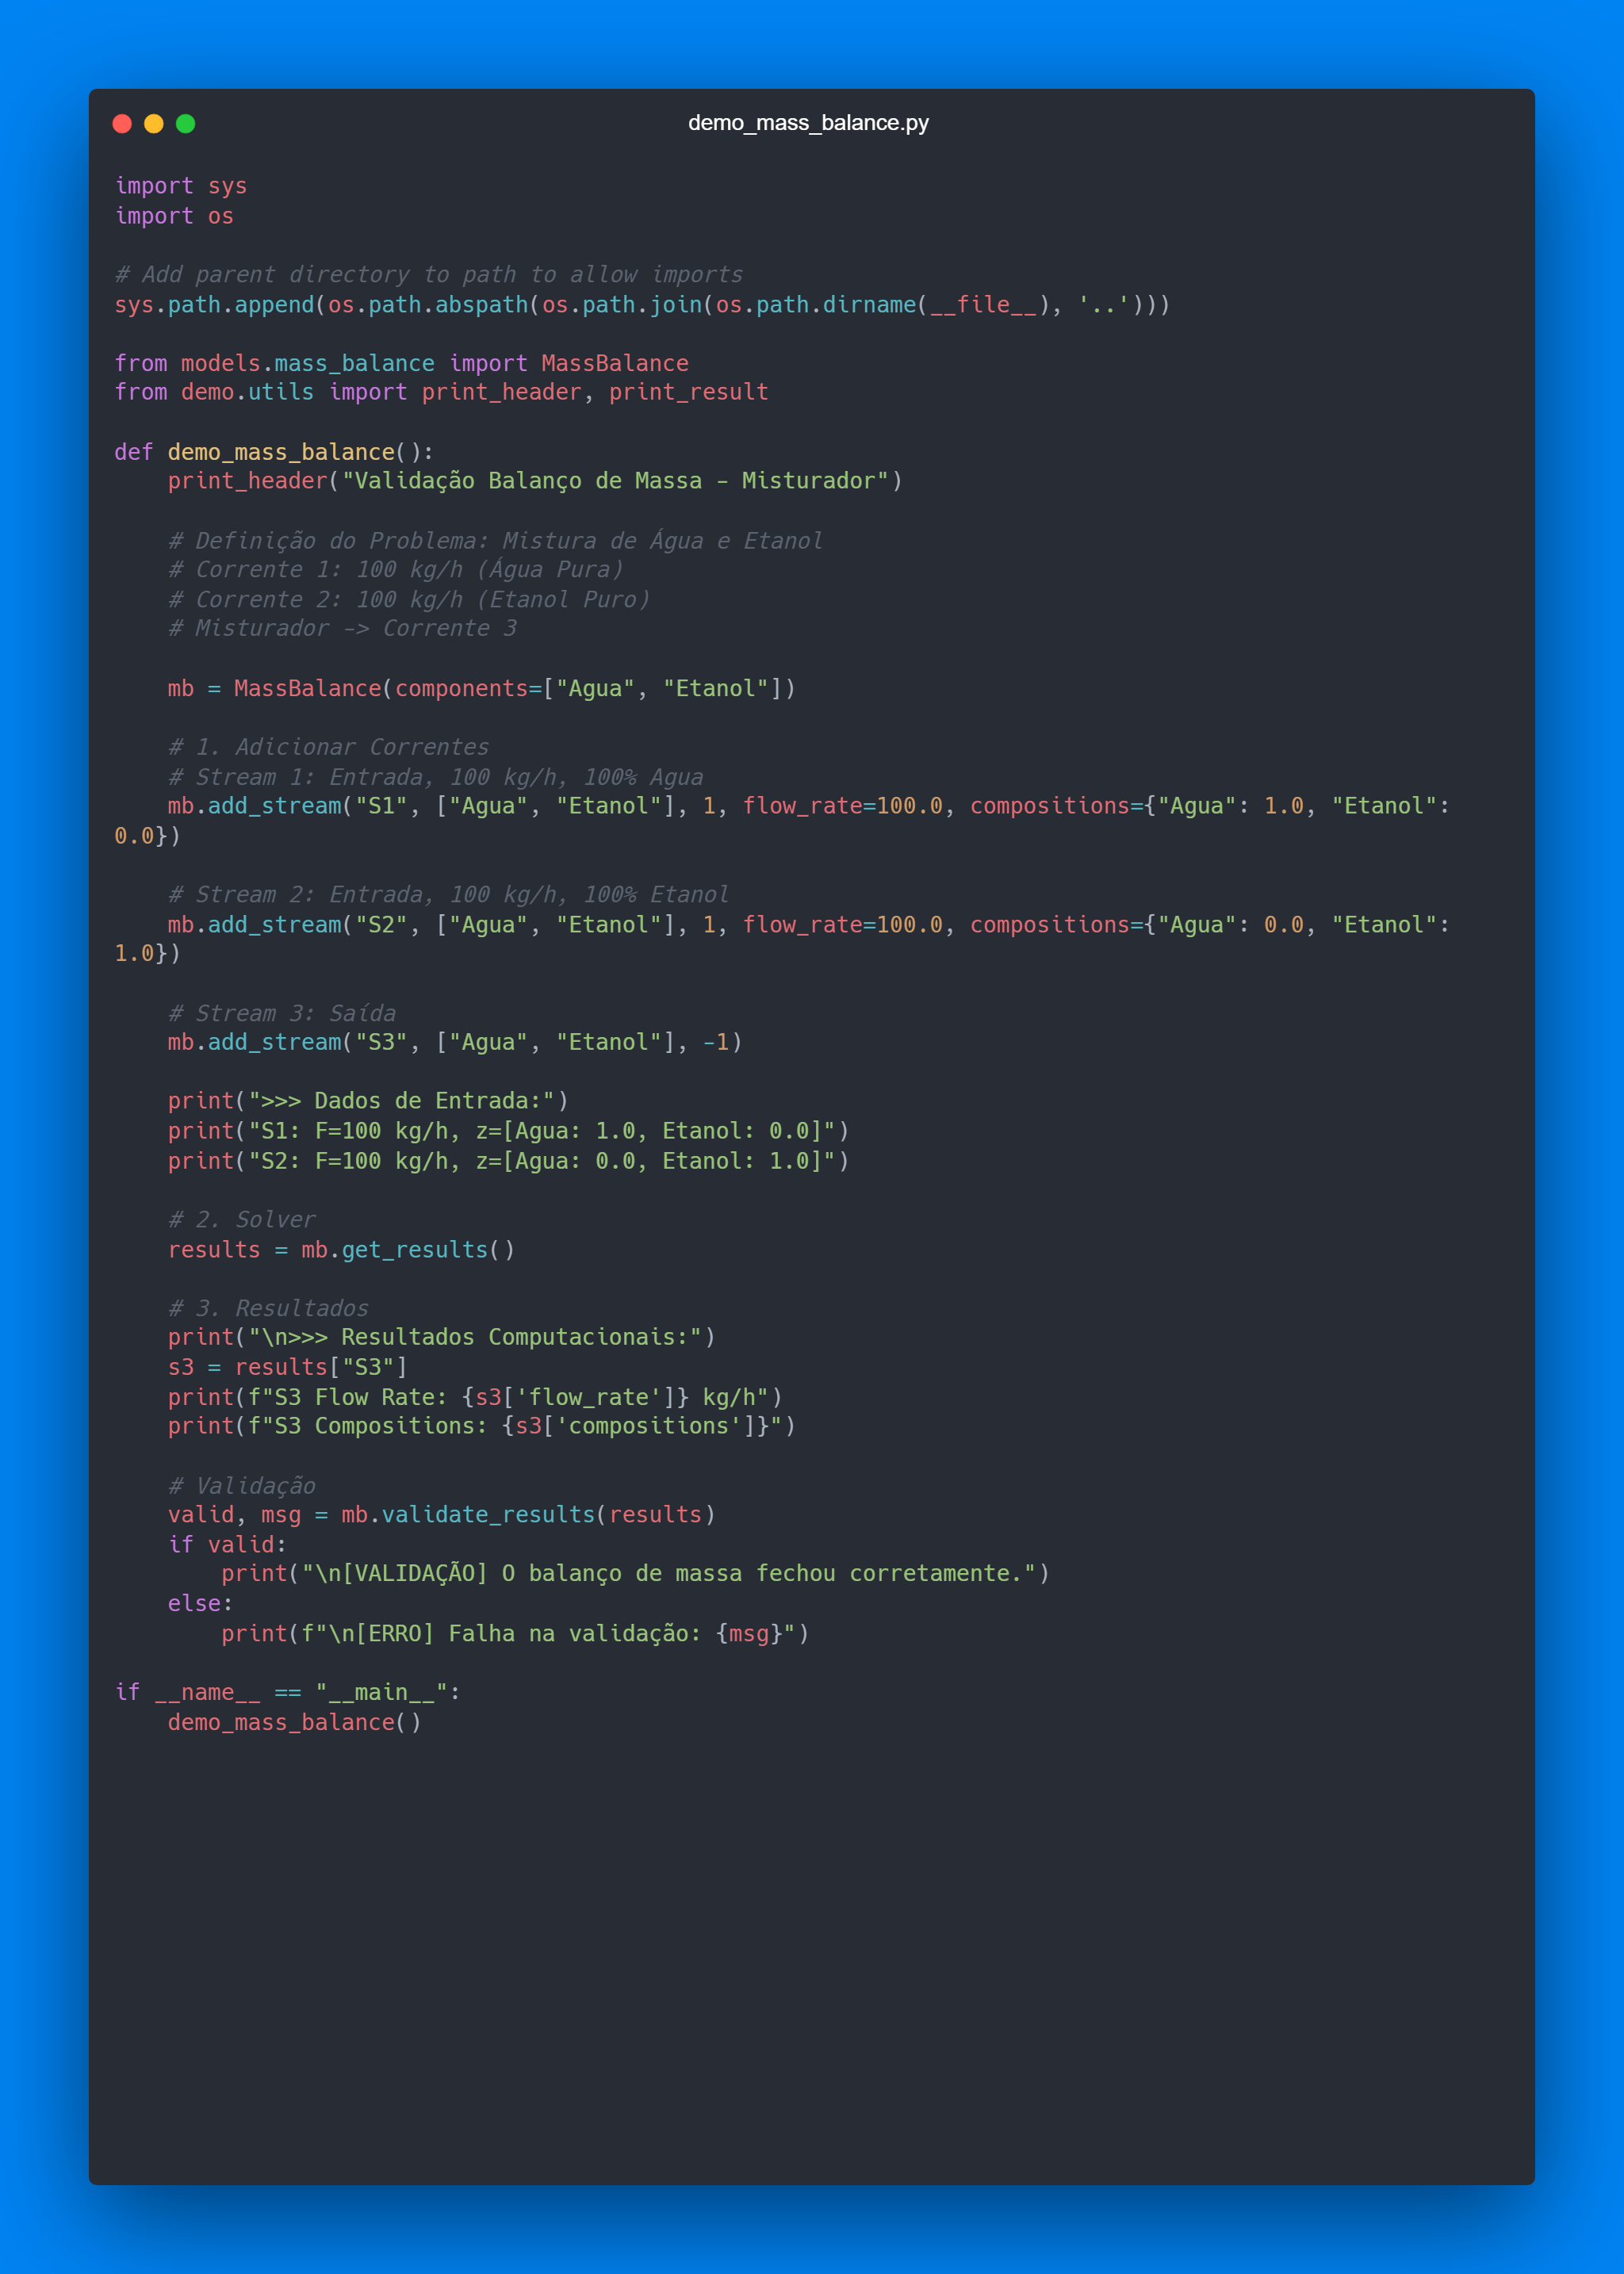
\includegraphics[width=\linewidth]{media/cap4_codigo_balanco_massa_misturador.png}
    \label{fig:code_mass_balance}
    \fonte{Elaboração própria (2026).}
\end{figure}

\begin{table}[H]
    \centering
    \caption{Validação Balanço de Massa (Misturador)}
    \begin{tabular}{lrrr}
        \toprule
        \textbf{Parâmetro} & \textbf{Cálculo Manual} & \textbf{\textit{Software}} & \textbf{Erro (\%)} \\
        \midrule
        Vazão $S3$ ($kg/h$) & 200,0 & 200,0 & 0,00 \\
        Fração Água $S3$ & 0,50 & 0,50 & 0,00 \\
        Fração Etanol $S3$ & 0,50 & 0,50 & 0,00 \\
        \bottomrule
    \end{tabular}
    \fonte{Elaboração própria (2026).}
\end{table}

\subsubsection{Reator de Conversão}

Neste caso, avalia-se a geração e consumo de espécies químicas em um sistema reacional simples.

\begin{itemize}
    \item \textbf{Reação:} $A \to B$ (Estequiometria 1:1).
    \item \textbf{Alimentação:} $100 \ mol/s$ de A puro.
    \item \textbf{Conversão ($X_A$):} $40\%$.
\end{itemize}

\textbf{Cálculo Manual:}
Pela estequiometria, para cada mol de A consumido, gera-se 1 mol de B.
\begin{equation}
    \label{eq:val_reaction_flow_a}
    F_{A,out} = F_{A,in}(1 - X_A) = 100(1 - 0,40) = 60 \ mol/s
\end{equation}
\begin{equation}
    \label{eq:val_reaction_flow_b}
    F_{B,out} = F_{A,in} X_A = 100(0,40) = 40 \ mol/s
\end{equation}
A vazão molar total permanece constante ($60+40=100$), resultando nas frações molares:
\begin{equation}
    \label{eq:val_reaction_mole_fractions}
    y_A = \frac{60}{100} = 0,6; \quad y_B = \frac{40}{100} = 0,4
\end{equation}

\textbf{Validação:}
O \textit{software} retornou: $F_{Product} = 100 \ mol/s$, com composição $z_A=0,6$ e $z_B=0,4$, confirmando a conservação de massa e estequiometria.

\subsubsection{Divisor de Corrente (\textit{Splitter})}

Simula-se uma operação de separação física onde uma corrente é dividida em duas (Reciclo e Produto) sem alteração de composição, típica em loops de reciclo.

\begin{itemize}
    \item \textbf{Entrada no Divisor:} $100 \ kg/h$ (mistura 50\% A, 50\% B).
    \item \textbf{Razão de Divisão (Reciclo):} $0,2$ ou $20\%$.
\end{itemize}

\textbf{Cálculo Manual:}
\begin{equation}
    \label{eq:val_recycle_flow_mass}
    F_{Reciclo} = 0,2 \cdot 100 = 20 \ kg/h
\end{equation}
\begin{equation}
    \label{eq:val_product_flow_mass}
    F_{Produto} = (1 - 0,2) \cdot 100 = 80 \ kg/h
\end{equation}
A composição deve permanecer inalterada: $z_A=0,5; z_B=0,5$ em ambas as saídas.

\textbf{Validação:}
Conforme apresentado na saída expandida do \textit{software} (Figura \ref{fig:code_mass_balance_exp}), os valores de vazão foram exatos ($20$ e $80 \ kg/h$) e a composição manteve-se constante, validando a lógica do divisor.

\begin{figure}[H]
    \centering
    \caption{Resultados expandidos da validação de Balanço de Massa (Misturador, Reator e \textit{Splitter})}
    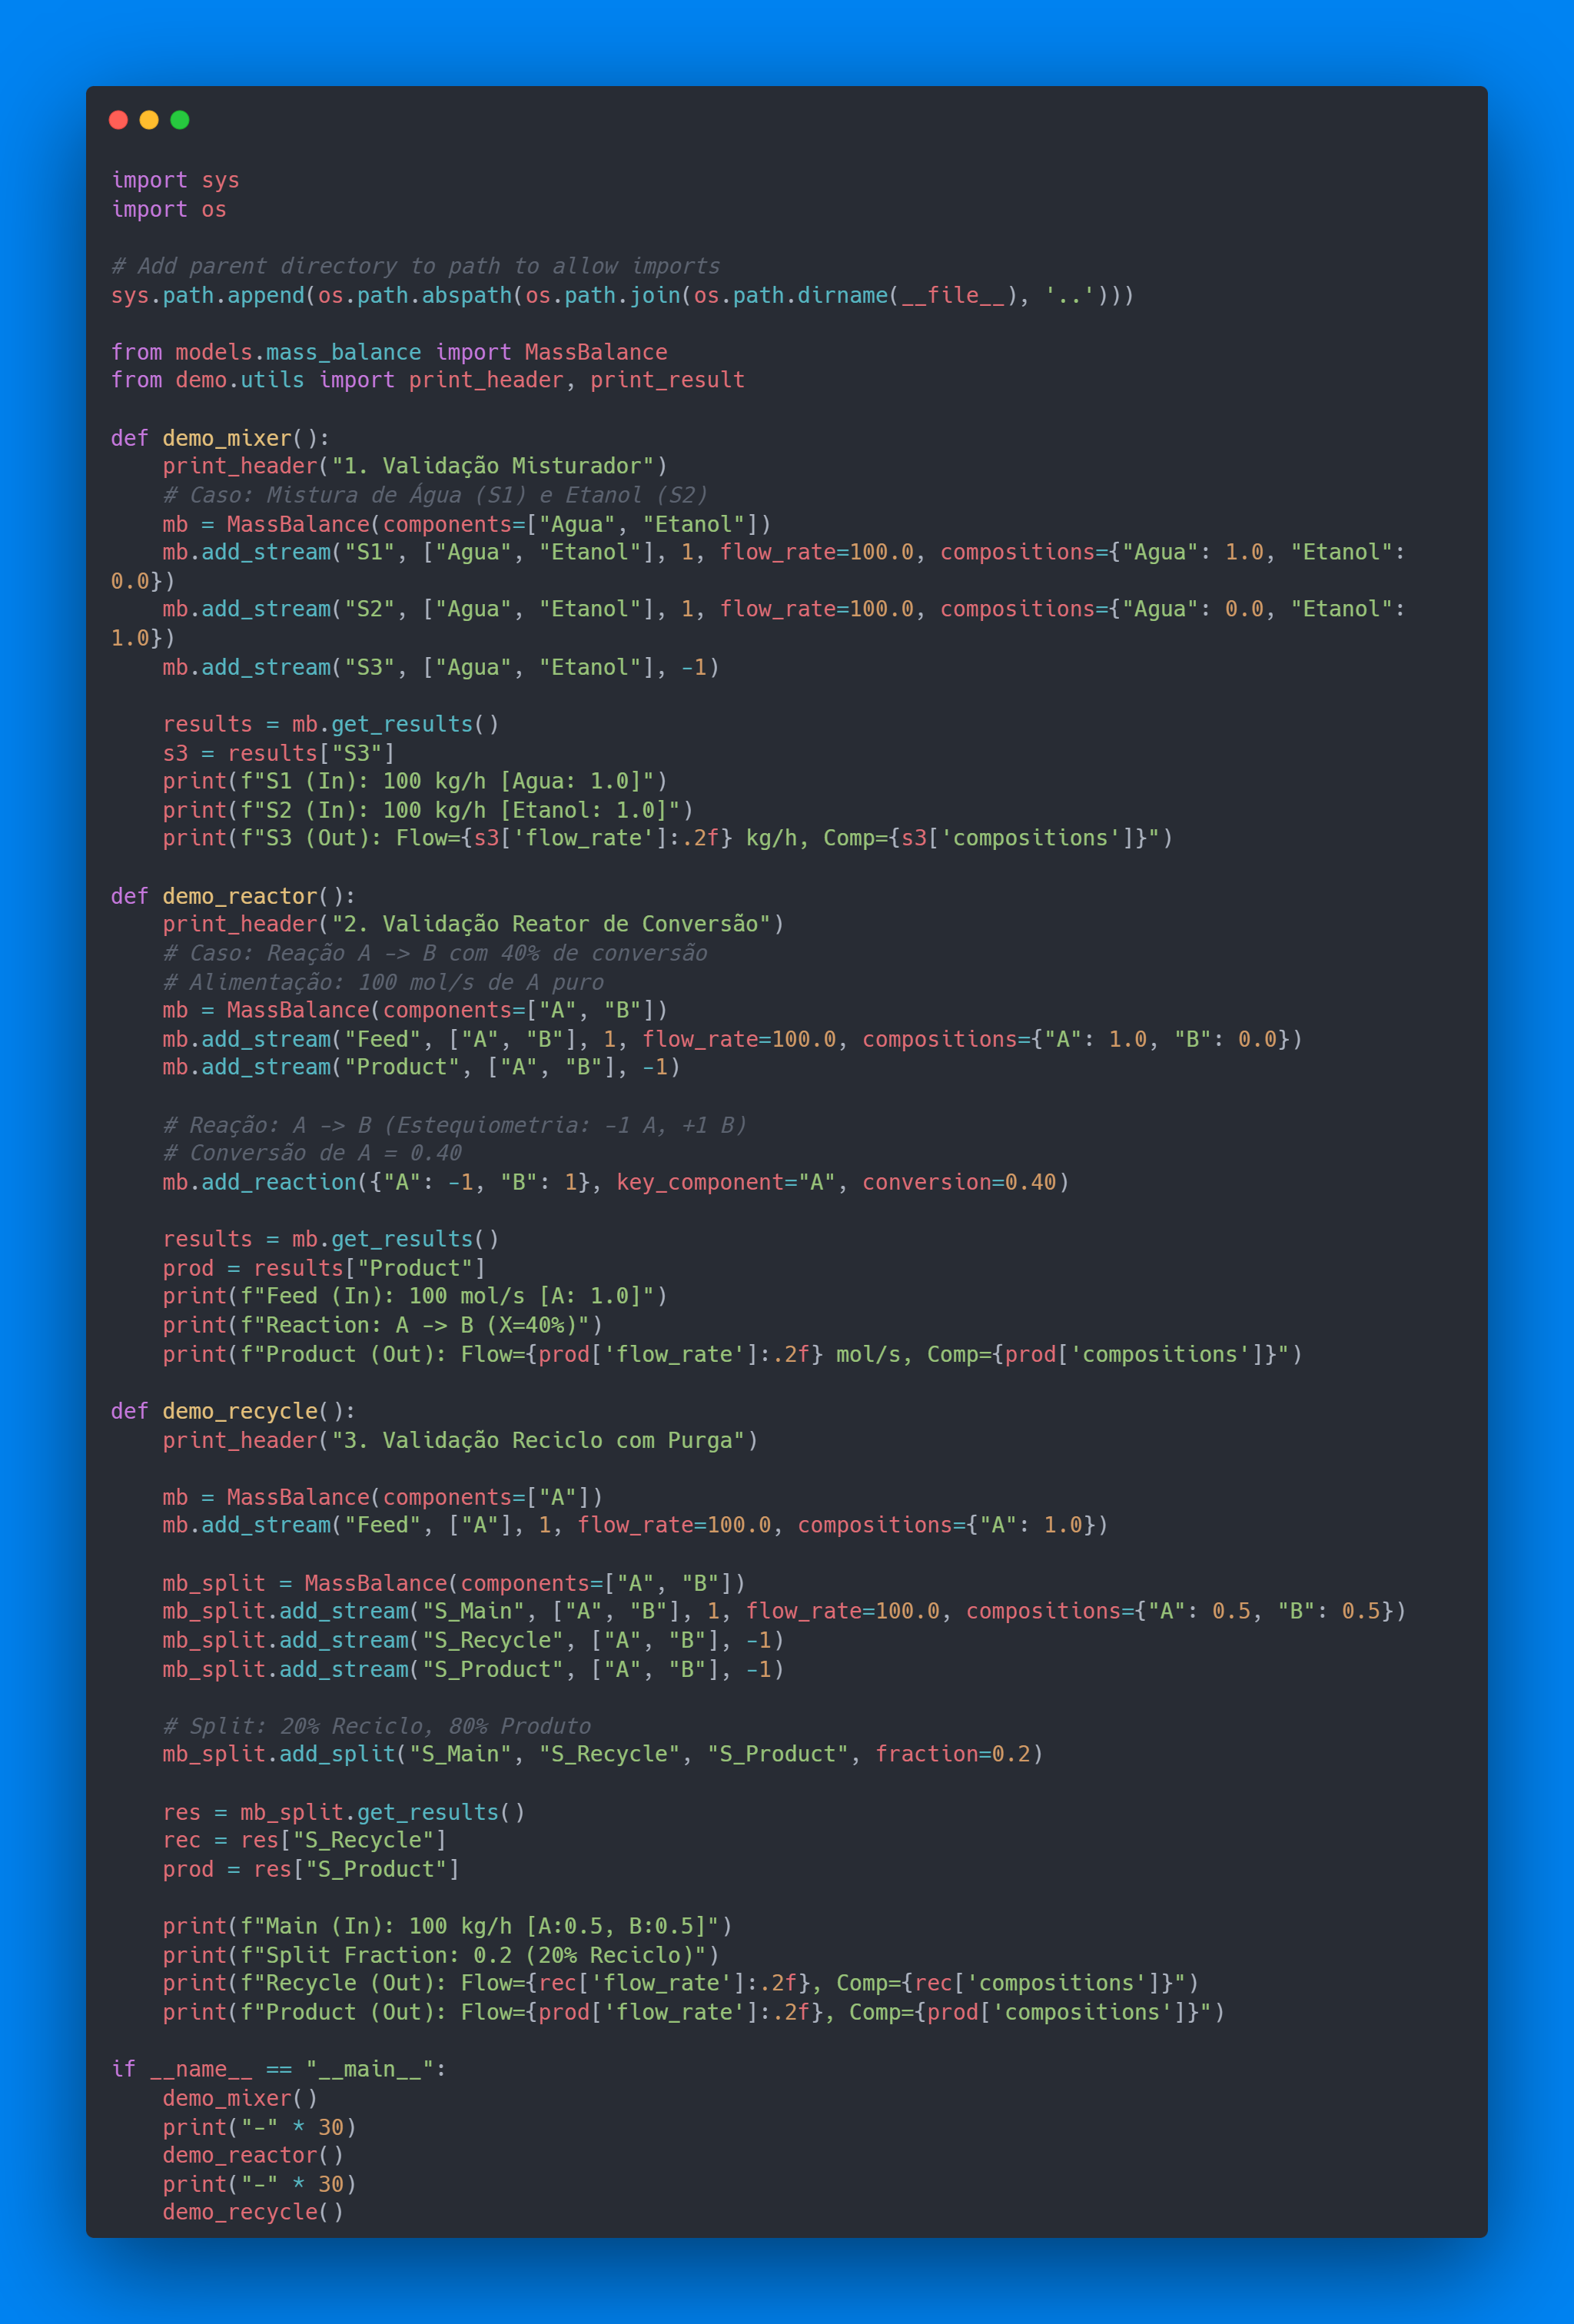
\includegraphics[width=\linewidth,height=0.85\textheight,keepaspectratio]{media/cap4_codigo_balanco_massa_expandido.png}
    \label{fig:code_mass_balance_exp}
    \fonte{Elaboração própria (2026).}
\end{figure}

\subsection{Tubulações}

O módulo de tubulações atua como um banco de dados de engenharia, fornecendo especificações padronizadas para acessórios, materiais e dimensões de tubos. A validação deste módulo consiste na verificação da conformidade dos dados retornados com as tabelas normativas padrão.

\subsubsection{Acessórios}

A função \textit{fittings()} retorna uma lista de todos os acessórios hidráulicos cadastrados no sistema. Esta funcionalidade permite que outros módulos (como o de Perda de Carga) validem a entrada de dados do usuário e utilizem os coeficientes corretos.

\subsubsection{Especificação de Acessórios}

A função \textit{fitting\_specifications(nome)} retorna os detalhes técnicos de um acessório, incluindo seu comprimento equivalente adimensional ($L_{eq}/D$) ou coeficiente de perda de carga ($K$).
Para validação, utilizou-se o acessório \textit{90 degrees Elbow long radius} (Cotovelo 90º Raio Longo).

\subsubsection{Composição}

A função \textit{compositions()} lista os materiais de tubulação disponíveis, associando-os às suas respectivas rugosidades absolutas, parâmetro crítico para o cálculo do Fator de Atrito de Darcy.

\subsubsection{Especificação da Composição}

A função \textit{composition\_specifications(nome)} retorna as propriedades de um material específico.
Para validação, verificou-se o material \textit{Commercial steel} (Aço comercial).

\subsubsection{\textit{Schedules}}

A função \textit{schedules()} fornece as classes de pressão/espessura disponíveis (ex: SCH40, SCH80), permitindo a seleção adequada conforme a norma ANSI/ASME B36.10M.

\subsubsection{Diâmetros}

A função \textit{diameters(schedule)} lista os diâmetros nominais (DN) disponíveis para uma determinada classe (\textit{schedule}).

\subsubsection{Especificação de Diâmetros}

A função \textit{diameter\_specifications(schedule, dn)} retorna as dimensões reais do tubo, incluindo diâmetro externo, espessura de parede e diâmetro interno (calculado).
Para validação, utilizou-se um tubo de \textit{Schedule} 40 com Diâmetro Nominal 50 (aprox. 2 polegadas).

\begin{table}[H]
    \centering
    \caption{Resumo dos contratos validados no módulo de tubulações}
    \label{tab:contratos-validacao-tubulacoes}
    \small
    \begin{tabular}{p{0.25\textwidth}p{0.28\textwidth}p{0.31\textwidth}}
        \hline
        \textbf{Contrato} & \textbf{Consulta validada} & \textbf{Evidência verificada} \\
        \hline
        Acessórios & \textit{fittings()} & Lista reutilizável para validação de entradas e perdas locais. \\
        Especificação de acessório & \textit{fitting\_specifications(}\\\textit{nome)} & Comprimento equivalente ou coeficiente $K$ do cotovelo de 90 graus de raio longo. \\
        Composição & \textit{compositions()} & Materiais disponíveis e suas rugosidades absolutas. \\
        Especificação de composição & \textit{composition\_}\\\textit{specifications(}\\\textit{nome)} & Propriedades do material Aço Comercial. \\
        Schedules & \textit{schedules()} & Classes de pressão e espessura, como SCH40 e SCH80. \\
        Diâmetros & \textit{diameters(schedule)} & Diâmetros nominais disponíveis para o SCH40. \\
        Especificação de diâmetro & \textit{diameter\_specifications(}\\\textit{schedule, dn)} & Diâmetro externo, espessura e diâmetro interno do tubo SCH40 DN50. \\
        \hline
    \end{tabular}
    \fonte{Autoria própria.}
\end{table}



\subsection{Reatores}

Esta seção apresenta a validação detalhada dos modelos de reatores \textit{CSTR} (\textit{Continuous Stirred-Tank Reactor}) e \textit{PFR} (\textit{Plug Flow Reactor}). Para garantir a precisão dos algoritmos, foram realizados cálculos manuais passo a passo para cenários de projeto e desempenho, comparando-os com os resultados obtidos pela ferramenta computacional.

Para todos os casos, adotou-se uma reação irreversível de primeira ordem $A \to B$ ocorrendo em fase líquida isotérmica, com os seguintes parâmetros globais:
\begin{itemize}
    \item Constante cinética da reação ($k$): $0,05 \ s^{-1}$
    \item Concentração inicial do reagente A ($C_{A0}$): $1000 \ mol/m^3$
    \item Vazão volumétrica de alimentação ($Q$ ou $v_0$): $0,01 \ m^3/s$
    \item Taxa molar de alimentação ($F_{A0}$): $10 \ mol/s$
\end{itemize}

\subsubsection{\textit{CSTR}: Reator Tanque Agitado Continuamente}

A equação de projeto (balanço molar) para um \textit{CSTR} operando em regime estacionário é a Equação \ref{eq:cstr_design}.

Para esta validação, a base dimensional segue os parâmetros globais acima; a cinética de primeira ordem gera $-r_A$ em $\mathrm{mol/(m^3\,s)}$ e as conversões permanecem adimensionais.

Para uma reação de primeira ordem em fase líquida (massa específica constante), a taxa de reação é dada por:
\begin{equation}
    -r_A = k C_A = k C_{A0} (1-X)
    \label{eq:val_rate_law}
\end{equation}

Substituindo na equação de projeto e sabendo que $F_{A0} = C_{A0} v_0$:
\begin{equation}
    V_{CSTR} = \frac{C_{A0} v_0 X}{k C_{A0} (1-X)} = \frac{v_0 X}{k (1-X)}
    \label{eq:val_cstr_vol_deriv}
\end{equation}

\textbf{Cálculo Manual (Design):}
Considerando uma conversão alvo de $X = 0,85$ ($85\%$):
\begin{equation}
    V_{manual} = \frac{0,01 \cdot 0,85}{0,05 \cdot (1 - 0,85)}
    \label{eq:val_cstr_vol_calc_1}
\end{equation}
\begin{equation}
    V_{manual} = \frac{0,0085}{0,05 \cdot 0,15} = \frac{0,0085}{0,0075} \approx 1,1333 \ m^3
    \label{eq:val_cstr_vol_calc_2}
\end{equation}

\textbf{Comparação com o Código:}
O módulo \textit{Reactor} foi executado com os mesmos parâmetros.
\begin{table}[H]
    \centering
    \caption{Validação \textit{CSTR} ($X=0,85$)}
    \begin{tabular}{lrrr}
        \toprule
        \textbf{Parâmetro} & \textbf{Cálculo Manual} & \textbf{\textit{Software}} & \textbf{Erro (\%)} \\
        \midrule
        Volume ($m^3$) & 1,1333 & 1,1333 & 0,0000 \\
        \bottomrule
    \end{tabular}
    \fonte{Elaboração própria (2026).}
\end{table}

Também validou-se o cálculo inverso (Desempenho), onde fornece-se $V=1,1333 m^3$ e espera-se $X=0,85$. O código retornou exatamente $0,8500$.

\subsubsection{\textit{PFR}: Reator Tubular}

A equação de projeto para um \textit{PFR} é obtida através do balanço diferencial de massa (Equação \ref{eq:pfr_design}).

Na validação do \textit{PFR}, $F_{A0}/(-r_A)$ tem unidade de volume ao combinar vazão molar com taxa molar de reação por volume de reator, e a integração ocorre sobre conversão adimensional.

Substituindo a cinética de primeira ordem:
\begin{equation}
    V = F_{A0} \int_{0}^{X} \frac{dX}{k C_{A0} (1-X)} = \frac{F_{A0}}{k C_{A0}} \int_{0}^{X} \frac{dX}{1-X}
    \label{eq:val_pfr_deriv_1}
\end{equation}

Como $\frac{F_{A0}}{C_{A0}} = v_0$:
\begin{equation}
    V = \frac{v_0}{k} \left[ -\ln(1-X) \right]_{0}^{X} = -\frac{v_0}{k} \ln(1-X)
    \label{eq:val_pfr_deriv_2}
\end{equation}

\textbf{Cálculo Manual (Design):}
Considerando uma conversão alvo de $X = 0,90$ ($90\%$):
\begin{equation}
    V_{manual} = -\frac{0,01}{0,05} \ln(1 - 0,90)
    \label{eq:val_pfr_calc_1}
\end{equation}
\begin{equation}
    V_{manual} = -0,2 \cdot \ln(0,10)
    \label{eq:val_pfr_calc_2}
\end{equation}
Sabendo que $\ln(0,10) \approx -2,302585$:
\begin{equation}
    V_{manual} = -0,2 \cdot (-2,302585) \approx 0,4605 \ m^3
    \label{eq:val_pfr_calc_3}
\end{equation}

\textbf{Comparação com o Código:}
\begin{table}[H]
    \centering
    \caption{Validação \textit{PFR} ($X=0,90$)}
    \begin{tabular}{lrrr}
        \toprule
        \textbf{Parâmetro} & \textbf{Cálculo Manual} & \textbf{\textit{Software}} & \textbf{Erro (\%)} \\
        \midrule
        Volume ($m^3$) & 0,4605 & 0,4605 & 0,0000 \\
        \bottomrule
    \end{tabular}
    \fonte{Elaboração própria (2026).}
\end{table}

\subsubsection{\textit{PFR} com Reciclo}

Em reatores com reciclo, parte da corrente de saída retorna à entrada. Para uma razão de reciclo $R$ (vazão reciclada / vazão fresca de alimentação), a conversão na entrada do reator ($X_{in}$) é diferente de zero, pois há mistura de reagentes frescos ($X=0$) com reagentes reciclados ($X=X_{out}$).

Na validação com reciclo, $R$, $X_{in}$ e a variável de integração $X$ permanecem adimensionais; $F_{A0}/(-r_A)$ define a escala de volume do reator.

A relação de balanço de massa no ponto de mistura fornece:
\begin{equation}
    X_{in} = \frac{R}{R+1} X_{out}
    \label{eq:val_recycle_xin}
\end{equation}

A equação de volume torna-se:
\begin{equation}
    V = (R+1) F_{A0} \int_{X_{in}}^{X_{out}} \frac{dX}{-r_A}
    \label{eq:val_recycle_vol_eq}
\end{equation}

Integrando para primeira ordem:
\begin{equation}
    V = (R+1) \frac{v_0}{k} \ln\left( \frac{1-X_{in}}{1-X_{out}} \right)
    \label{eq:val_recycle_vol_int}
\end{equation}

\textbf{Cálculo Manual (Design):}
Considerando uma conversão de saída $X_{out} = 0,90$ e razão de reciclo $R = 2,0$.

Passo 1: Calcular $X_{in}$.
\begin{equation}
    X_{in} = \frac{2,0}{2,0 + 1} \cdot 0,90 = \frac{2}{3} \cdot 0,90 = 0,60
    \label{eq:val_recycle_xin_calc}
\end{equation}

Passo 2: Calcular o Volume.
\begin{equation}
    V_{manual} = (2 + 1) \cdot \frac{0,01}{0,05} \cdot \ln\left( \frac{1 - 0,60}{1 - 0,90} \right)
    \label{eq:val_recycle_vol_calc_1}
\end{equation}
\begin{equation}
    V_{manual} = 3 \cdot 0,2 \cdot \ln\left( \frac{0,40}{0,10} \right) = 0,6 \cdot \ln(4)
    \label{eq:val_recycle_vol_calc_2}
\end{equation}
Sabendo que $\ln(4) \approx 1,38629$:
\begin{equation}
    V_{manual} = 0,6 \cdot 1,38629 \approx 0,8318 \ m^3
    \label{eq:val_recycle_vol_calc_3}
\end{equation}

\textbf{Comparação com o Código:}
\begin{table}[H]
    \centering
    \caption{Validação \textit{PFR} com Reciclo ($R=2,0; X=0,90$)}
    \begin{tabular}{lrrr}
        \toprule
        \textbf{Parâmetro} & \textbf{Cálculo Manual} & \textbf{\textit{Software}} & \textbf{Erro (\%)} \\
        \midrule
        Volume ($m^3$) & 0,8318 & 0,8318 & 0,0000 \\
        \bottomrule
    \end{tabular}
    \fonte{Elaboração própria (2026).}
\end{table}

Os testes confirmam que as rotinas computacionais implementam corretamente as equações diferenciais e algébricas fundamentais da engenharia de reações, incluindo cenários complexos de integração numérica com limites variáveis como no caso do reciclo.
